\documentclass[12pt, openany]{report}
\usepackage[utf8]{inputenc}
\usepackage[T1]{fontenc}
\usepackage{amsmath,amsfonts,amssymb}
\usepackage{amssymb}
\usepackage{multicol}
\usepackage[a4paper,left=2.5cm,right=2.5cm,top=2.5cm,bottom=2.5cm]{geometry}
\usepackage[english]{babel}
\usepackage{libertine}
\usepackage{graphicx}
\usepackage{wrapfig}
\usepackage{algorithm}
\usepackage{algpseudocode}
\usepackage{float}
\usepackage{enumitem}
\usepackage{pythonhighlight}
\usepackage[]{titletoc}
\usepackage{empheq}
\usepackage{titlesec}
\usepackage{mathpazo}
\usepackage{xfrac}
\usepackage{textcomp}
\usepackage{mathtools}
\usepackage{caption}
\usepackage{tabularray}
\usepackage{subcaption}
\usepackage[bottom]{footmisc}
\usepackage{pdfpages}
\usepackage{tabularx}
\usepackage{amsthm}
\usepackage[skins]{tcolorbox}
\titleformat{\chapter}[display]
  {\normalfont\bfseries}{}{0pt}{\Huge}
\usepackage{hyperref}
\newcommand{\hsp}{\hspace{20pt}}
\newcommand{\HRule}{\rule{\linewidth}{0.5mm}}
\newcommand{\R}{\mathbb{R}}
\newcommand{\C}{\mathbb{C}}
\theoremstyle{definition}
\newtheorem{thm}{Theorem}[chapter]
\newtheorem{definition}[thm]{Definition}
\newtheorem{lem}[thm]{Lemma}

\hbadness=100000
\begin{document}
\begin{titlepage}
    \begin{sffamily}
    \begin{center}
        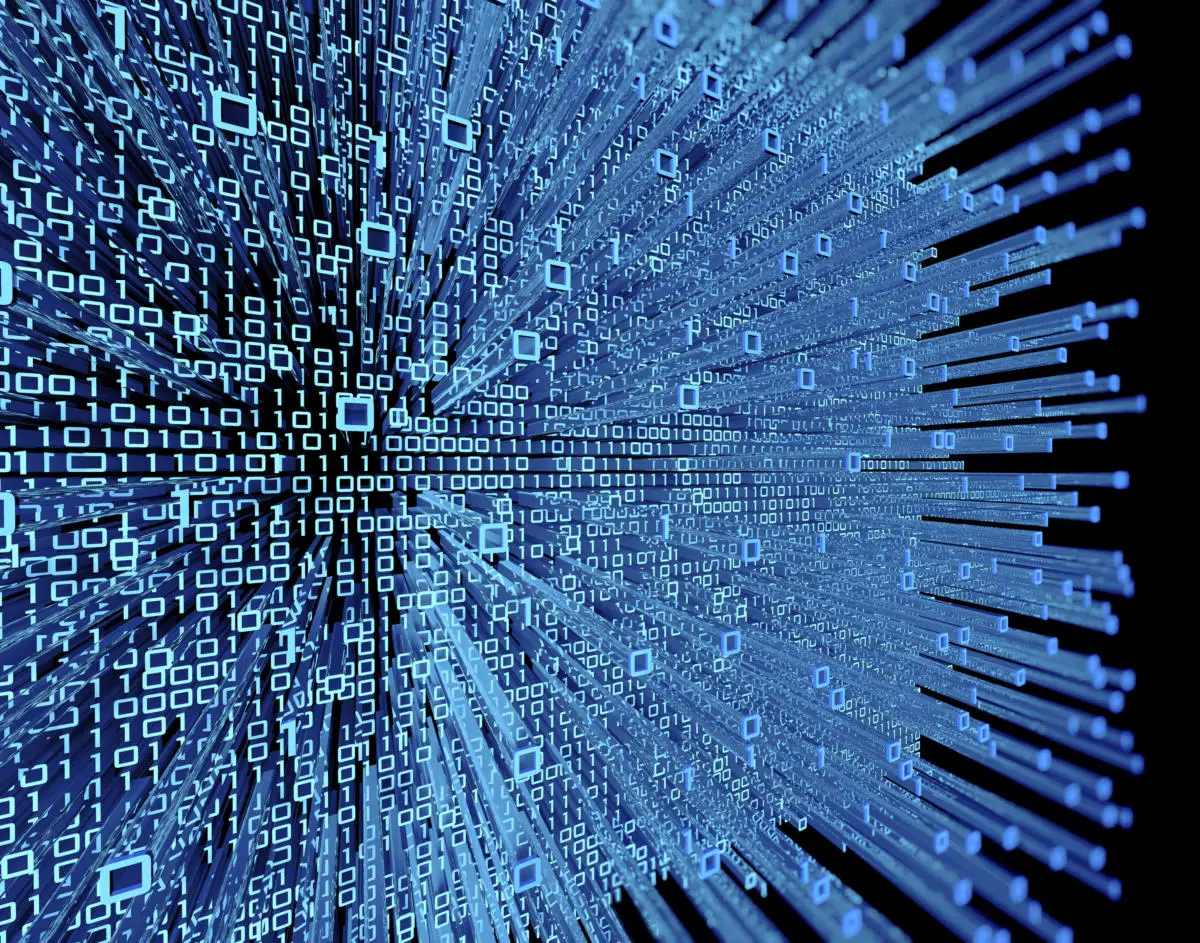
\includegraphics[scale=0.25]{img/page_de_garde.png} \\[1cm]
        \HRule \\[0.4cm]
        { \huge \bfseries LINMA2710 Scientific Computing \\[0.4cm] }
    
        \HRule \\[1.5cm]
        \textsc{\LARGE Simon Desmidt}\\[1cm]
        \vfill
        \vspace{2cm}
        {\large Academic year 2024-2025 - Q2}
        \vspace{0.4cm}
         
        
\includegraphics[width=0.15\textwidth]{img/epl.png}
        
        UCLouvain\\
    
    \end{center}
    \end{sffamily}
\end{titlepage}

\setcounter{tocdepth}{1}
\tableofcontents
\chapter{Single Instruction Multiple Data (SIMD)}
\chapter{Shared-Memory Multiprocessing}
\section{How memory works}
\subsection{Memory hierarchy} 
To store the data that it will use, the CPU uses memory. Memory is hierarchical like a pyramid. The higher it is, the faster it goes, but the less space there is.
\begin{figure}[H]
    \centering
    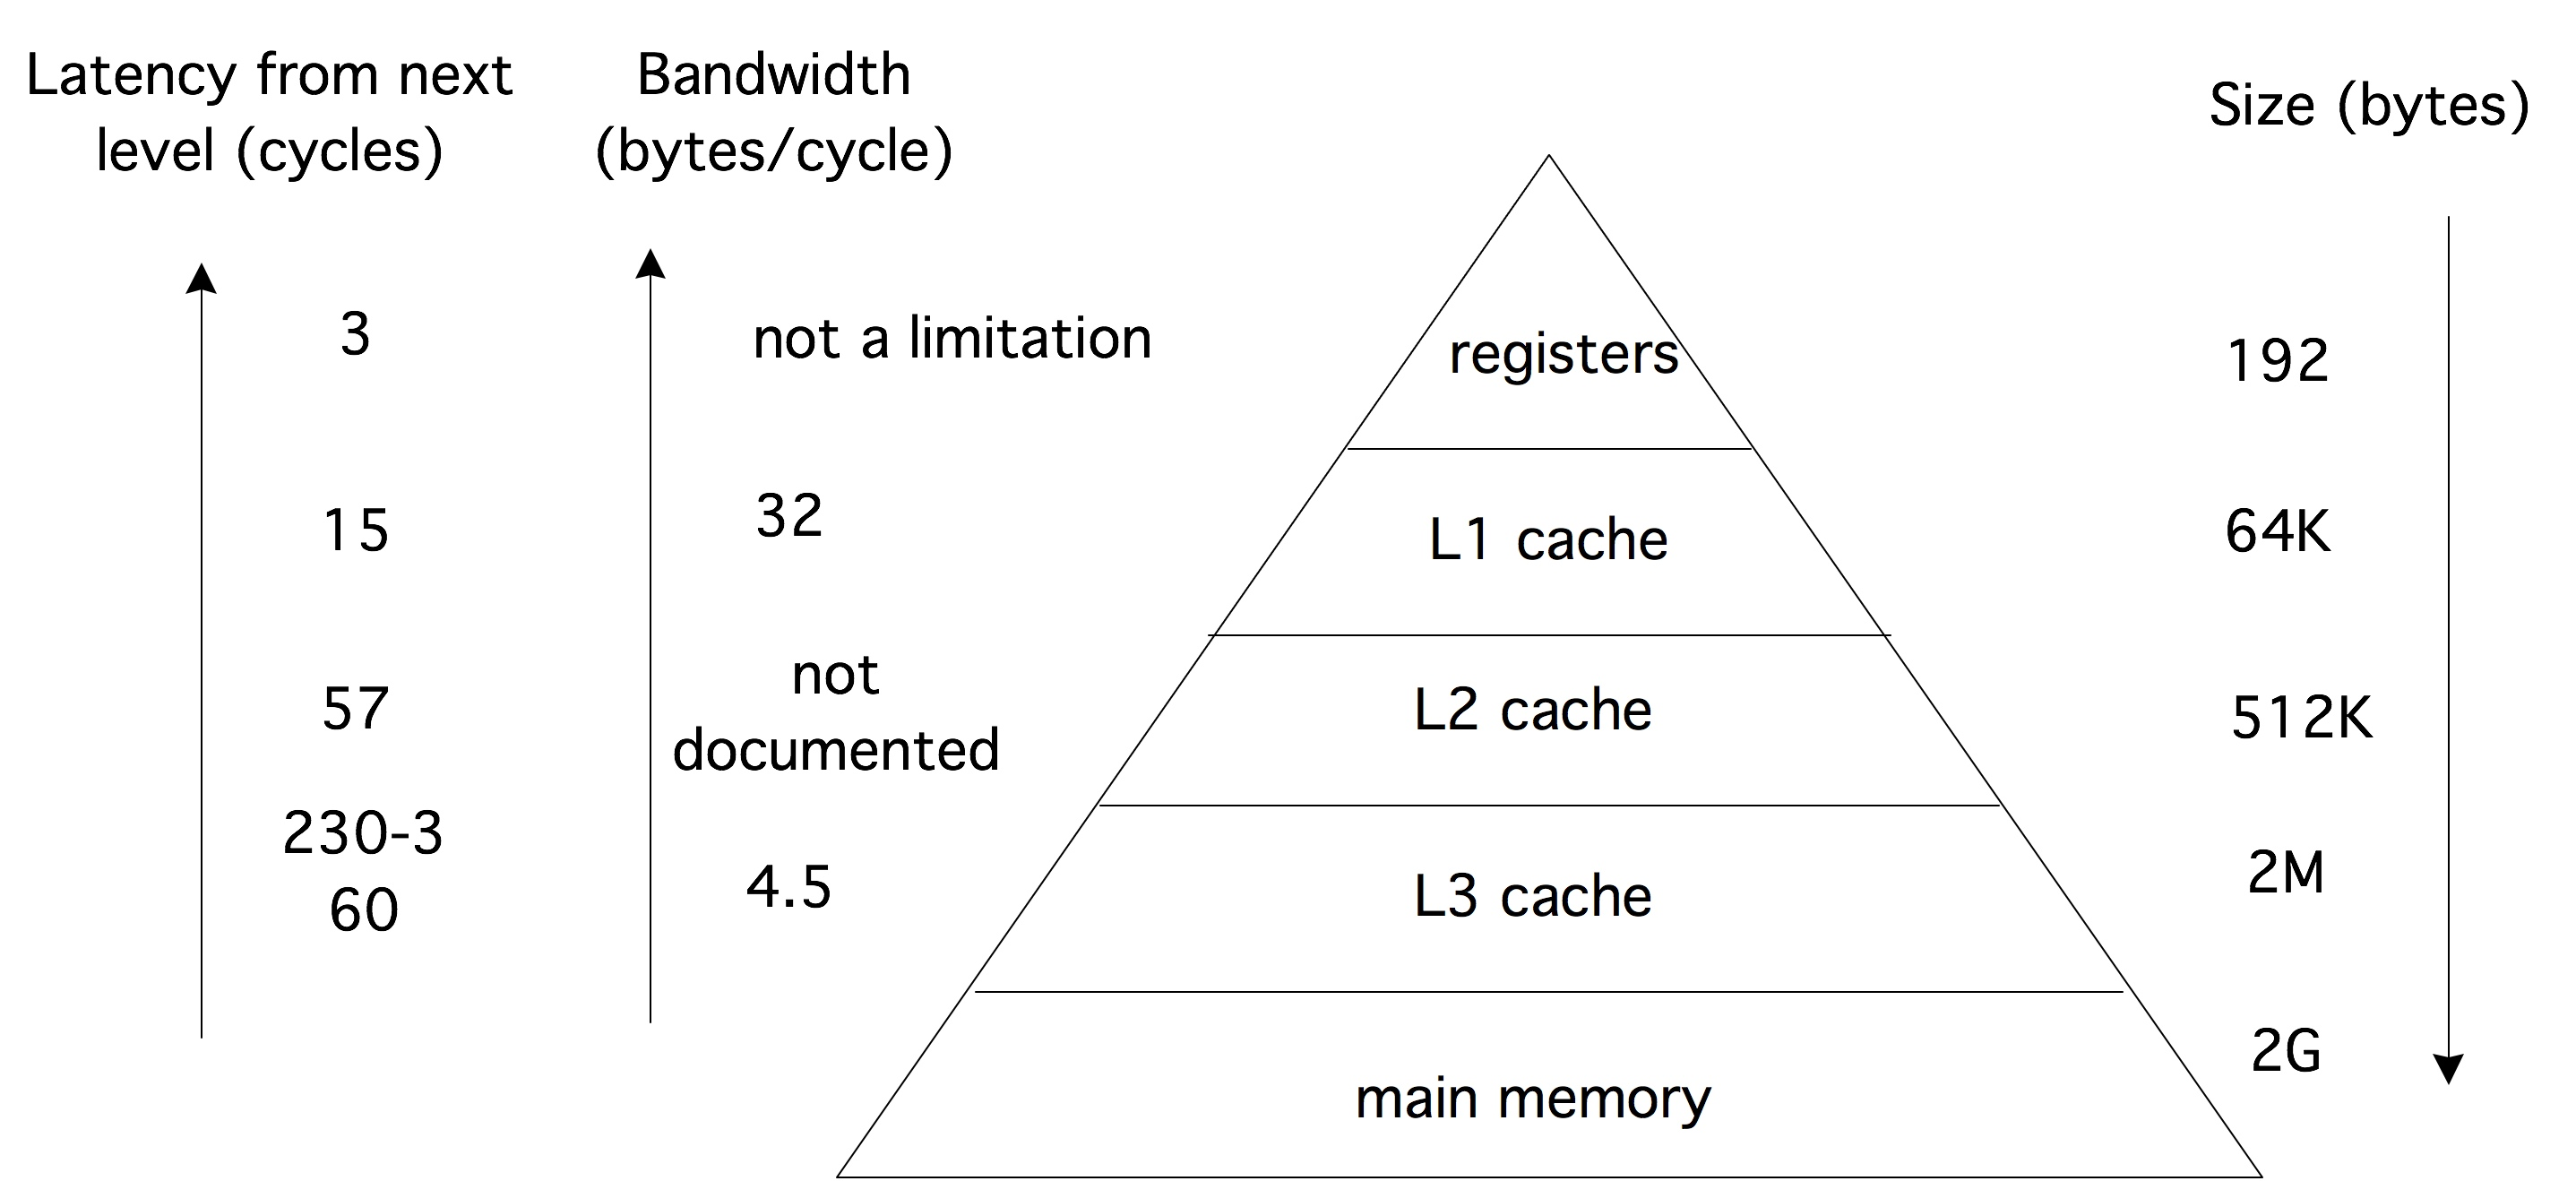
\includegraphics[scale=0.15]{img/memory_layout.jpeg}
    \caption{Memory hierarchy}
    \label{fig:memory_hierarchy}
\end{figure}
First we need to define a cycle. It's an unit of time that is defined like this: $cycle = \frac{1}{\text{CPU freq}}$. For example, for the CPU \textit{AMD Ryzen 5 5600X}, the maximum frequency is $4.6 GHz$, so the cycle is $cycle = \frac{1}{4.6 GHz} \approx 0.217 ns$. The \textbf{bandwidth} is the number of bytes that can be transferred in one cycle. And the \textbf{latency} is the number of cycle required to access a level of memory. There's also the \textbf{latency} but for a number of bytes, it's formula is $\alpha + \beta n$ where $\alpha$ is the level latency, $\beta$ is the inverse of the bandwidth and $n$ is the number of bytes.\\
\begin{tabularx}{\textwidth}{|c|X|X|X|X|X|}
	\hline
	Level & Level \newline Latency $[cycle]$  & Bandwidth $[bytes/cycle]$ & Size & What \newline is stored & example \\
	\hline
	Register & $3$ & No limit & $\pm 192B$ & "Immeditate" data for the CPU & Results of addition, memory address\\
	\hline
	Cache L1 & $15$ & $32-64$ & $\pm 64KB$ & Instructions and \newline "Immeditate" data & Local variable\\
	\hline
	Cache L2 & $57$ & $16-32$ & $\pm 512KB$ & Data used recently & Data struct, code part\\
	\hline
	Cache L3 & $230-360$ & $4-10$ & $\pm 64MB$ & Data shared between core& Global variable\\
	\hline
	RAM & $300-500$ & $9-50GB/s$ & $+4GB$ & Running programs & Running software, open document\\
	\hline
	Disks & $+10^6$ & Usually $\leq 3GB/s$ & $+128GB$ & Persistent data & Document, OS, etc\\
	\hline
\end{tabularx}
\subsection{Caches lines and prefetching}
A \textbf{cache line} is a small fixed-size contiguous block of memory, usually $64$ or $128$ bytes. It's not necessarly stored in the cache. We use them to organize the memory, because it is easier to deal with fixed size block. When the CPU need to access a memory location, it loads the entire cache line into the cache of the CPU.
If the wanted data is not in the cache, there will be a \textbf{cache miss}. After that the CPU will load the entire cache line into the cache.\\
The \textbf{prefetching} is the fact that the CPU will load the cache line that is next to the one that is needed. It's because of the spacial locality. Spacial locality is the reason why we use cache lines. For example, if we store an array of data, it may use some space greater than one cache line so for precaution, the CPU will load the next cache line too. And so we save time, by anticipating.\\
For example of the importance of data locality we have:
\begin{itemize}
	\item \textbf{Temporal locality}: If a data is used frequently, we will keep it in the cache.
	\item \textbf{Spacial locality}: If a data is used, the data next to it could be usefull too.
\end{itemize}
\subsection{Arithmetic intensity}
The \textbf{arithmetic intensity} is a concept in performance analysis for memory-bound and compute-bound programs.
Let's consider a programs that do $o$ arithmetic operations and $m$ memory operations, we define:
\begin{itemize}
	\item \textbf{Arithmetic intensity}: 
	\begin{equation} 
		a = \frac{o}{m}
	\end{equation}
	It helps to find if the program is limited by a compute-bound or memory-bound.
	\item \textbf{Arithmetic time}: 
	\begin{equation} 
		t_{arith} = \frac{o}{\text{CPU freq}}
	\end{equation}
	It's the time needed to performs $o$ operations.
	\item \textbf{Memory transfer time}:
	\begin{equation} 
		t_{mem} = \frac{m}{\text{bandwidth}} = \frac{o}{a \times \text{bandwidth}}
	\end{equation}
	It's the time needed to do $m$ memory operations. 
\end{itemize}
The overall performance of a program is thus defined by the wrost component of the PC, and so we get the \textbf{time per iteration}:
\begin{equation}
	\min \left( \frac{t_{arith}}{o},\frac{t_{mem}}{o} \right)
\end{equation}
With some algebra, we can find the \textbf{number of operations per second}:
\begin{equation}
	\max \left( \text{CPU freq}, a \times \text{bandwidth} \right)
\end{equation}
\subsection{The roofline model}
\subsection{cache hierarchy for a multi-core CPU}
\end{document}